%\alex{\textbf{NOTE: The paper outline is still {\it very} rough, and I expect to re-order
%many sections, largely in attempt to keep the focus on the system.}}

\begin{figure}
	\centering
	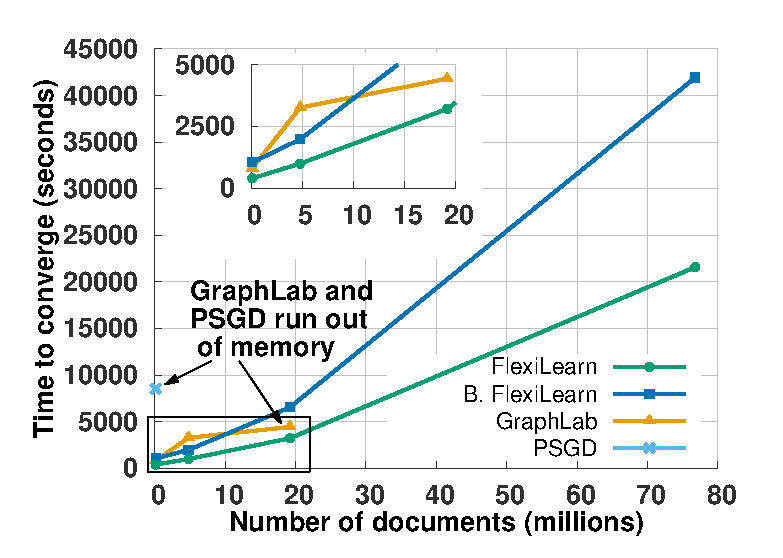
\includegraphics[width=0.8\columnwidth]{fig2/lda_datasize.eps}
	\caption{Scalability comparison for topic modeling}
	\label{fig:crownjewel}
\end{figure}

In recent years, the amount of data being produced and stored throughout the
world has exploded.  From science to e-commerce to news to social networking,
we, as a culture, are spending more time and money producing uniquely digital
content and recording elements of our physical world online for posterity and
analysis.  With this big data boom, the focus is often on the size of the data
- ``LHC produced 13 petabytes \ldots of data in
2010\footnote{\url{http://www.nature.com/news/2011/110119/full/469282a.html}}''
and ``500+terabytes of new data ingested into [Facebook] databases every
day\footnote{\url{http://gigaom.com/2012/08/22/facebook-is-collecting-your-data-500-terabytes-a-day/}}.''
While handling all of this data is an important challenge and lots of work has
focused on scaling to large datasets, this misses an important part of the
picture - we are also recording more data about {\em more things}: ``300
million photos uploaded per day [to Facebook]'' and there are more than 400
million tweets sent per
day\footnote{\url{http://articles.washingtonpost.com/2013-03-21/business/37889387_1_tweets-jack-dorsey-twitter}}.
The challenge now becomes not just using all of the data, but also
understanding all of these items.

Traditional DBMS's have focused on analyzing big data and can perform numerous
aggregate queries.  But what happens when the questions we want to ask are more
complex, like what are the topics of millions of news articles?
Machine learning has focused on asking such complex questions and understanding
large datasets for many years, but the research often ignores the challenge of
scaling to models over many
millions or even billions of items, e.g. finding the topics of billions of
webpages, removing noise from the many images upoaded online, or clustering
users in a billion node social network.  In each of these cases, the issue is not
just the size of the data but also the number of items we need to model and
understand.  Even if we distribute our dataset across many machines, the model
of topics for 100 million documents (news articles or webpages) across even 100
topics would take over 35 gigabytes just to store in memory.  

In this paper we describe a new system, \method, for answering such complex
questions about modern massive datasets.  Informally and generally,
the problem we are solving is:\\ 
\textbf{Given:} A database of relations between different objects\\
\textbf{Find:} A model of those objects which best matches those relationionships.\\
As an example, for the special case of topic modelling this can be framed, again informally, as:\\
\textbf{Given:} A database of documents for which we know the use of different words in different documents\\
\textbf{Find:} The probability of each document being about a particular topic,
and for each topic the probability that a word is used when discussing that topic.\\
We define our problem formally as a minimization problem over a class of functions in
Section \ref{sec:problem}.  

In order to answer a variety of such complex questions, \method focuses on a
new abstraction for relational data that enables easy partitioning and
distribution of both the dataset and model across a cluster of machines.  This
abstraction for relational data is flexible enough to answer a wide variety of
common machine learning queries.  In this paper we describe the following
contributions:
\begin{enumerate}[noitemsep,topsep=1.5pt,parsep=1.5pt,partopsep=1.5pt]
	\item \textbf{Scalability:} Our system scales to model billions of items
		using massive datasets.  We are particularly efficient in our memory
		usage, enabling us to scale beyond current state of the art systems.
	\item \textbf{Versatility:} \method can answer a wide variety of complex
		machine learning queries, often with even higher accuracy than other
		systems.  We demonstrate our effectiveness on topic modeling,
		dictionary learning for de-noising images, and mixed membership
		stochastic block models for clustering users in a network.
	\item \textbf{Speed:} We use new techniques for running over barriers to
		not waste computational time even when waiting stragglers in the cluster.
		This lets \method converge to the final answer faster than
		competitors.
	\item \textbf{Portability:} Because of Apache's Hadoop
		and HDFS ubiquity in industry, we build our system on top of these
		frameworks.  This makes it extremely easy to run the system without
		having to modify your cluster.
\end{enumerate}

In Section \ref{sec:problem} we formally define our problem.
In Section \ref{sec:mdAbstract} we explain our scalable abstraction for the
model and data, and give the high level overview of computation under this
abstraction in a cluster.  In Section \ref{sec:learning} we give the background
on different learning techniques, such as gradient based learning, for modeling
our data.  In Section \ref{sec:complexQues} we describe how our system can
answer a wide variety of complex questions, such as what is the probability of
a webpage being about a set of topics.  In Section \ref{sec:overBarriers} we
explain how we can continue performing valuable computation even while waiting
for stragglers to catch up, thus enabling our system to converge to the solution
quickly.  In Section \ref{sec:implementation} we give the details of how we
implemented the system on Hadoop.  In Section \ref{sec:applications} we
describe a few different applications of our system and in Section
\ref{sec:experiments} we describe our experimental setup.  In Section
\ref{sec:eval} we evaluate our system against other state of the art systems.
Finally in Section \ref{sec:related} we give a survey of the related work, and we
conclude in Section \ref{sec:conclusion}.
